\documentclass[12pt]{article}
\usepackage[top=1in,bottom=1in,left=0.75in,right=0.75in,centering]{geometry}
\usepackage{fancyhdr}
\usepackage{epsfig}
\usepackage[pdfborder={0 0 0}]{hyperref}
\usepackage{palatino}
\usepackage{wrapfig}
\usepackage{lastpage}
\usepackage{color}
\usepackage{ifthen}
\usepackage[table]{xcolor}
\usepackage{graphicx,type1cm,eso-pic,color}
\usepackage{hyperref}
\usepackage{amsmath}
\usepackage{wasysym}
\usepackage{latexsym}
\usepackage{amssymb}

\def\course{CS 4102: Algorithms}
\def\homework{Module 9 - Network Flow and Ford-Fulkerson}
\def\semester{Fall 2021}

\newboolean{solution}
\setboolean{solution}{false}

% add watermark if it's a solution exam
% see http://jeanmartina.blogspot.com/2008/07/latex-goodie-how-to-watermark-things-in.html
\makeatletter
\AddToShipoutPicture{%
\setlength{\@tempdimb}{.5\paperwidth}%
\setlength{\@tempdimc}{.5\paperheight}%
\setlength{\unitlength}{1pt}%
\put(\strip@pt\@tempdimb,\strip@pt\@tempdimc){%
\ifthenelse{\boolean{solution}}{
\makebox(0,0){\rotatebox{45}{\textcolor[gray]{0.95}%
{\fontsize{5cm}{3cm}\selectfont{\textsf{Solution}}}}}%
}{}
}}
\makeatother

\pagestyle{fancy}

\fancyhf{}
\lhead{\course}
\chead{Page \thepage\ of \pageref{LastPage}}
\rhead{\semester}
%\cfoot{\Large (the bubble footer is automatically inserted into this space)}

\setlength{\headheight}{14.5pt}

\newenvironment{itemlist}{
\begin{itemize}
\setlength{\itemsep}{0pt}
\setlength{\parskip}{0pt}}
{\end{itemize}}

\newenvironment{numlist}{
\begin{enumerate}
\setlength{\itemsep}{0pt}
\setlength{\parskip}{0pt}}
{\end{enumerate}}

\newcounter{pagenum}
\setcounter{pagenum}{1}
\newcommand{\pageheader}[1]{
\clearpage\vspace*{-0.4in}\noindent{\large\bf{Page \arabic{pagenum}: {#1}}}
\addtocounter{pagenum}{1}
\cfoot{}
}

\newcounter{quesnum}
\setcounter{quesnum}{1}
\newcommand{\question}[2][??]{
\begin{list}{\labelitemi}{\leftmargin=2em}
\item [\arabic{quesnum}.] {#2}
\end{list}
\addtocounter{quesnum}{1}
}

\definecolor{red}{rgb}{1.0,0.0,0.0}
\newcommand{\answer}[2][??]{ 
\ifthenelse{\boolean{solution}}{
\color{red} #2 \color{black}}
{\vspace*{#1}}
}

\definecolor{blue}{rgb}{0.0,0.0,1.0}

\begin{document}

\section*{\homework}

\question[3]{
Take the following flow-network and run the Ford-Fulkerson algorithm on it. Once you are done, write the following items in your response:

\begin{itemize}
	\item Write the original / starting residual graph $G_f$ for this network BEFORE execution of Ford-Fulkerson begins. This should be an \emph{Adjacency Matrix}
	\item Write out the final / ending residual graph $G_f$ after Ford-Fulkerson completes. This should be an \emph{Adjacency Matrix} and make sure to include \emph{backflow edges}.
	\item What is the final maximum flow $f$ for this Graph?
\end{itemize}
}

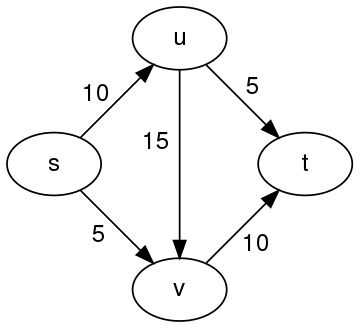
\includegraphics[width=0.4\textwidth]{flowNetwork}

\answer[0.1in]{...}

\question[3]{
Consider the flow network you see below (the bolded edges the first augmenting path that Ford-Fulkerson will discover). What is the \textbf{maximum} number of iterations that Ford-Fulkerson could make (i.e., what is the most number of times DFS could run). Explain how this maximum could be reached and why it is a major issue.
}

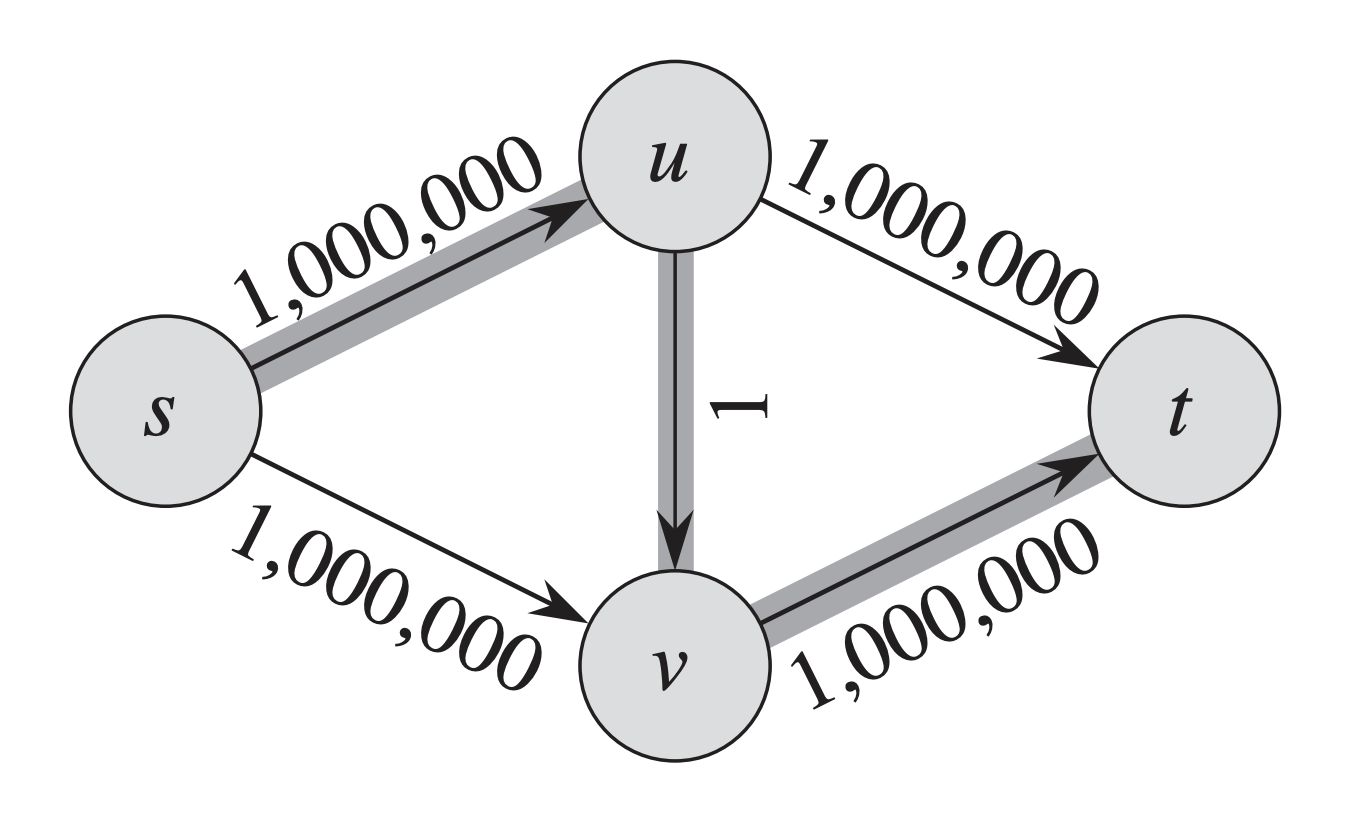
\includegraphics[width=0.4\textwidth]{slowNetwork}

\answer[0.15in]{...}

\question[3]{
Suppose we want to take a \emph{flow-network} as input, and return a set of at most $|E|$ augmenting paths that produce the maximum flow on that network. Describe an algorithm to do this. \emph{Hint: Find the maximum flow using any number of augmenting paths first, then try to reverse engineer how to reach that flow with at most $|E|$ augmenting paths.}
}


\end{document}